
\begin{figure*}
    \centering
    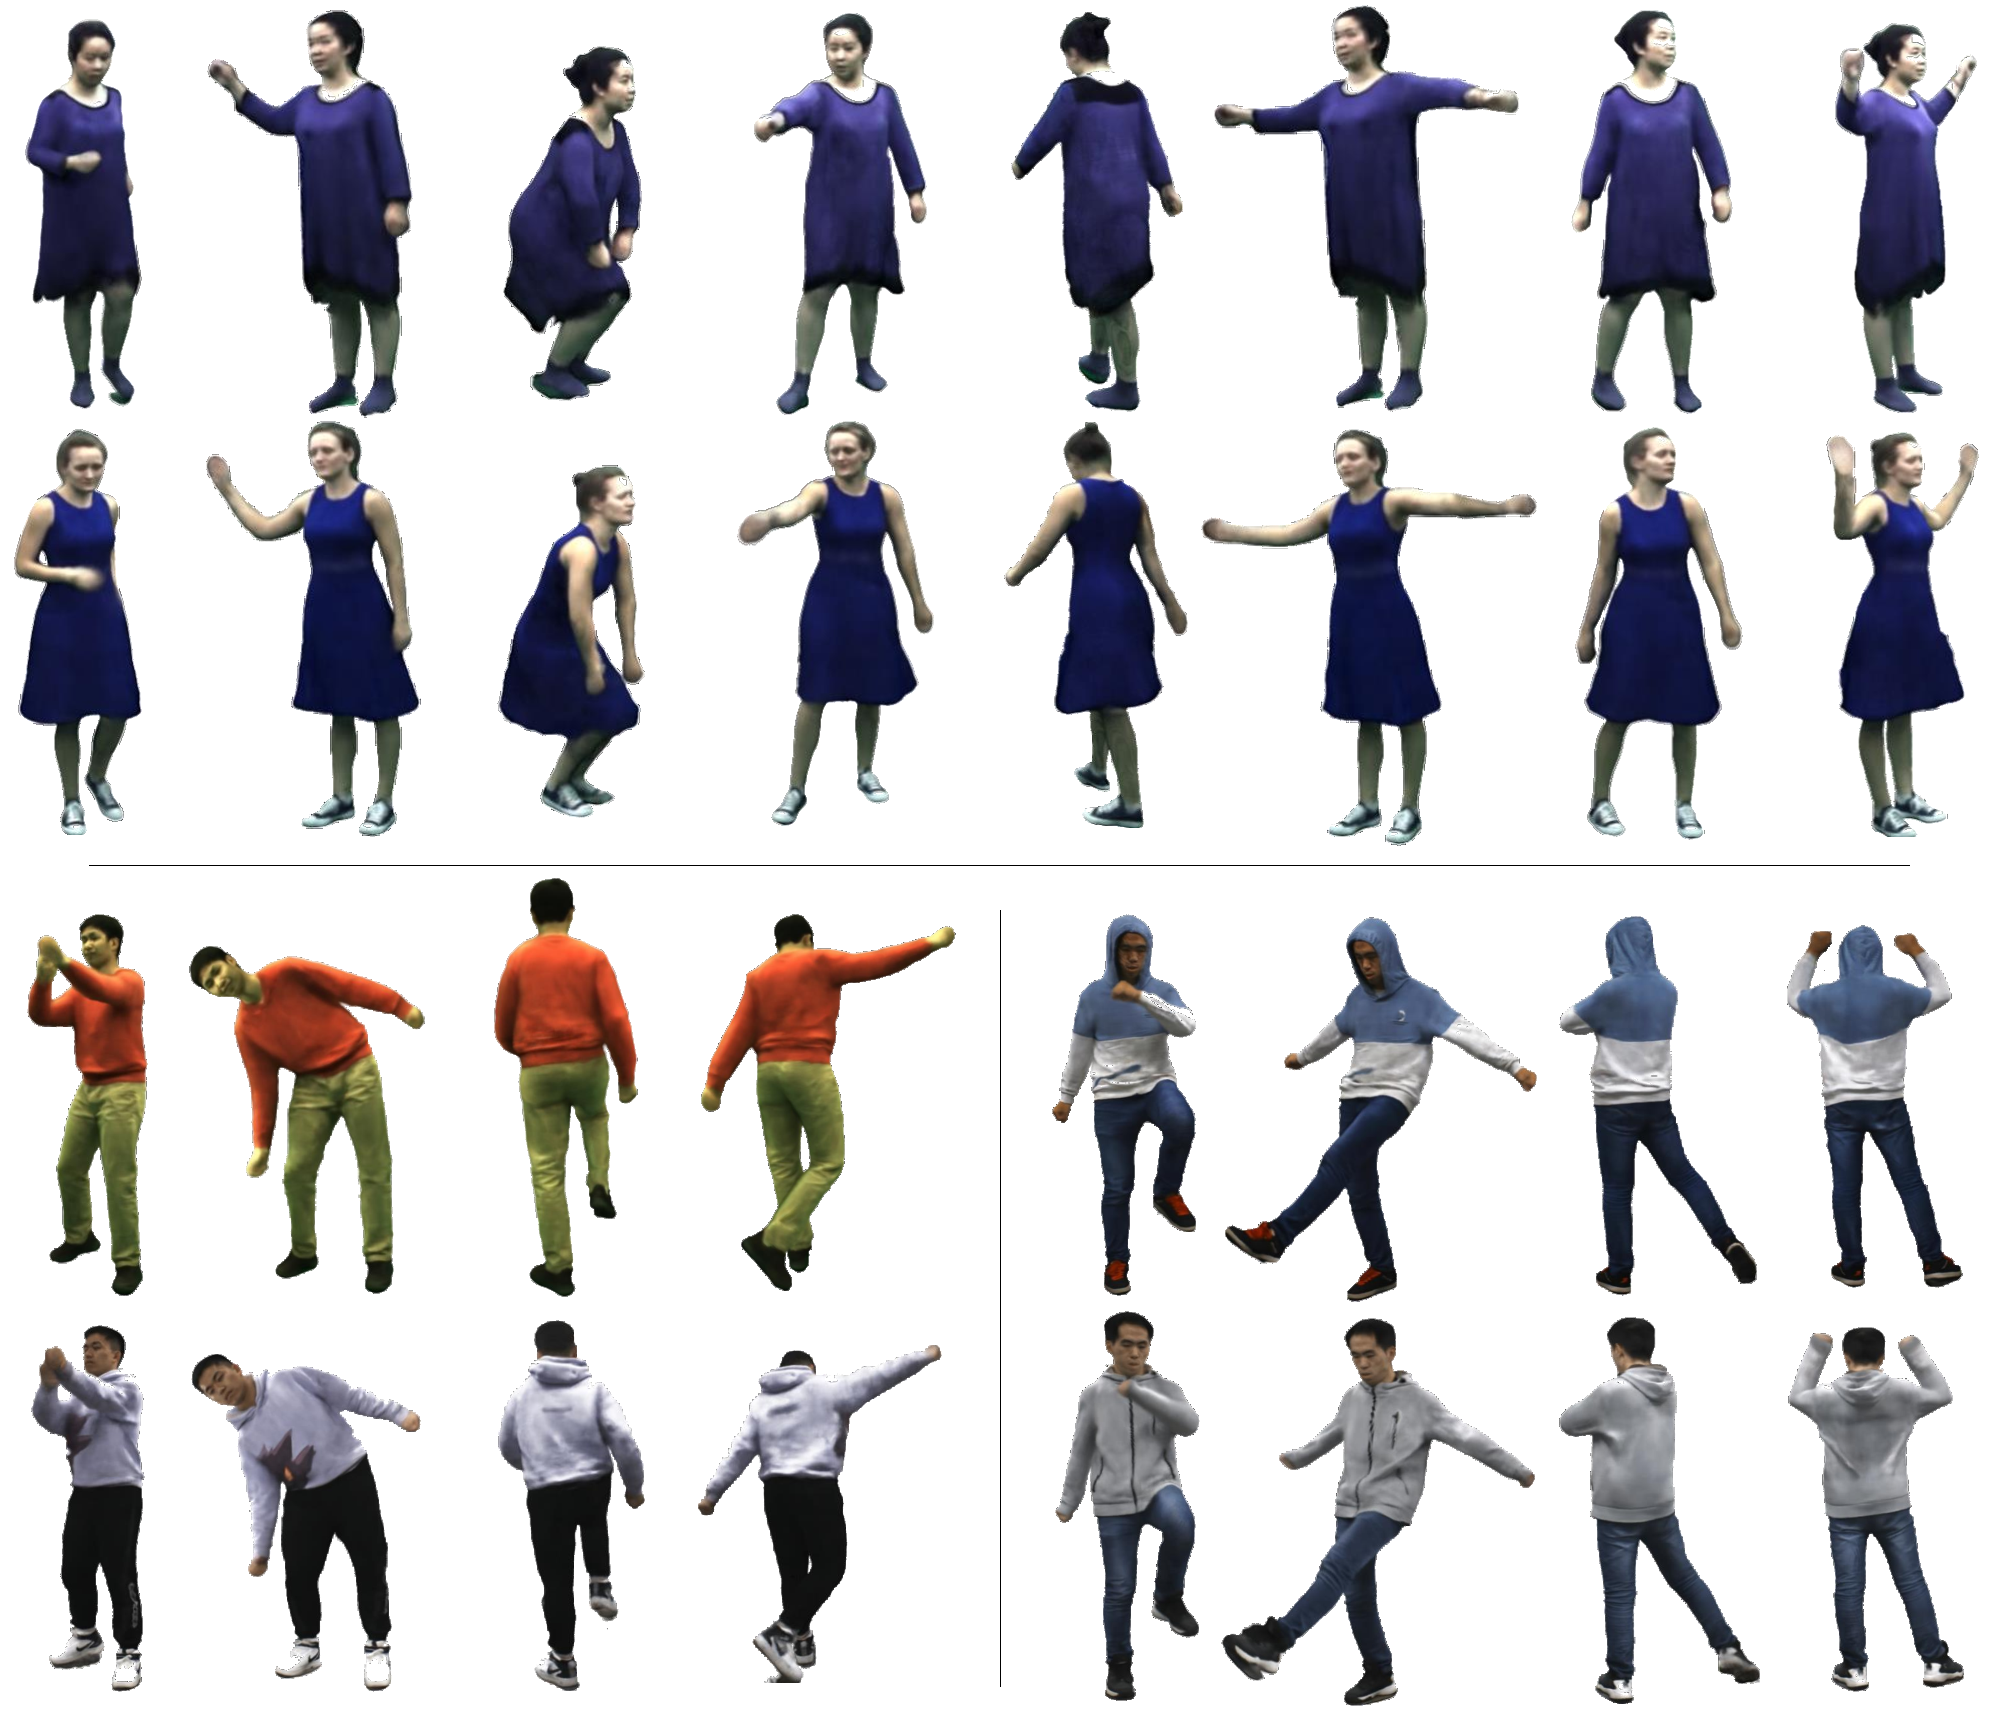
\includegraphics[width=0.98\linewidth]{results_middle}
    \caption{\textbf{Example results of our method.} We train our network on various datasets and show the novel pose synthesis results. }
    \label{fig:results}
\end{figure*}





\begin{figure}
    \centering
    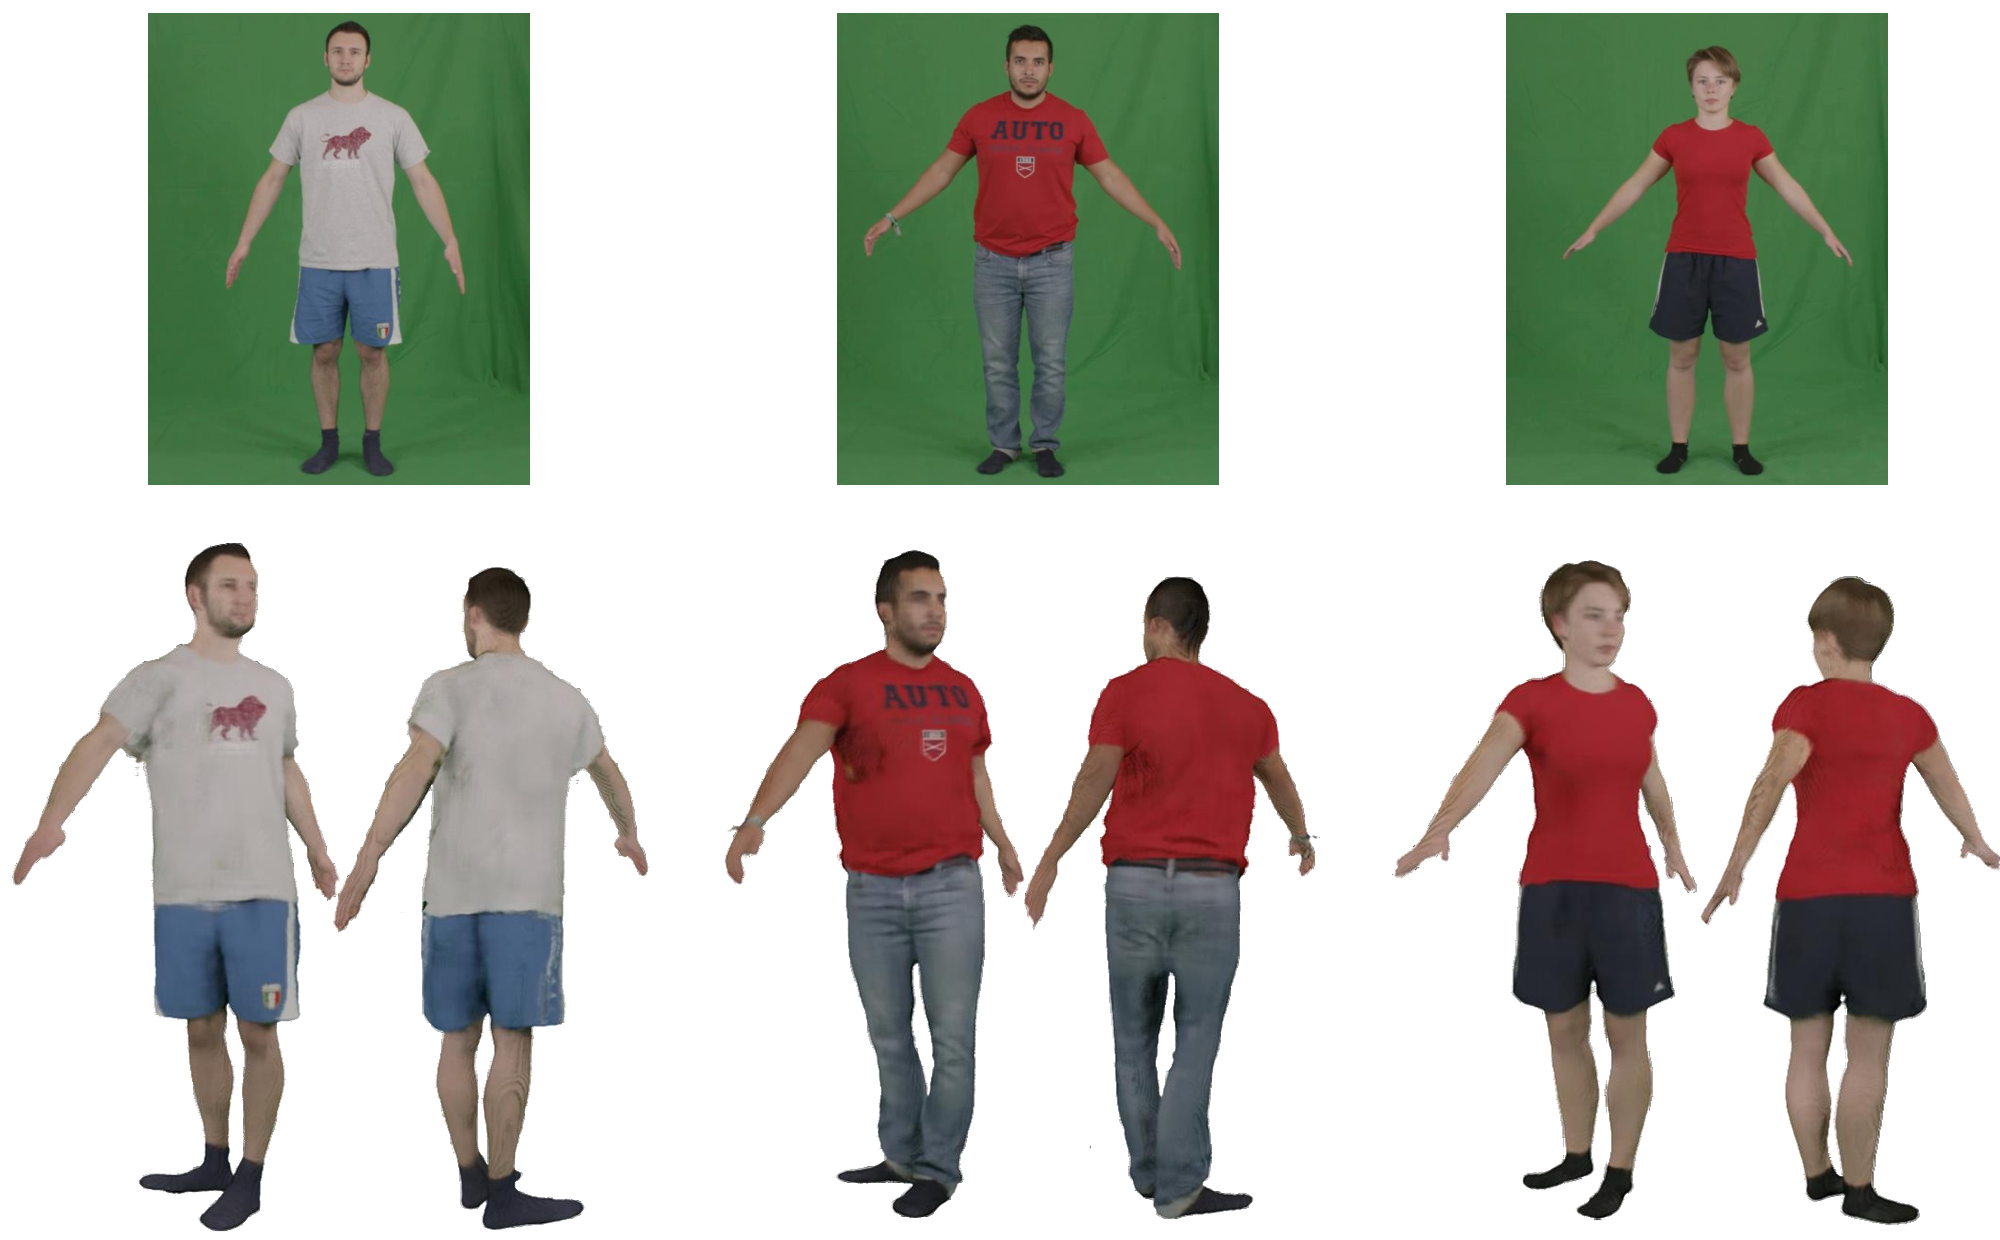
\includegraphics[width=1.0\linewidth]{singleview2}
    \caption{\textbf{Our results on PeopleSnapshot dataset.} Given a monocular video recording a person rotating in an A-pose (top), our method is able to create a human avatar that supports novel pose generation and free view synthesis (bottom). }
    \label{fig:singleview}
\end{figure}



\section{Experiments}
\label{sec:experiments}
\noindent\textbf{Dataset and Metrics. } 
For evaluation and comparison with baseline methods, we mainly use the following dataset: 
(1) Two dress sequences from \cite{habermann2021realtimeDDC}, which are captured using 100 cameras but we manually select 20 views among them for computational efficiency; (2) One sweater sequences from \cite{habermann2020deepcap} captured with 10 cameras; (3) Two sequences from ZJU-MoCap~\cite{peng2021neuralbody} captured with 23 cameras; and (4) three multi-view sequences collected by ourselves with 24 cameras\footnote{Data collection and disclosure have been consented by the volunteers. }. For quantitative evaluation, we use two standard metrics: peak signal-tonoise ratio (PSNR) and structural similarity index (SSIM).
More details about data collection and preprocessing can be found in the \textit{Supp.Mat.}.


\subsection{Results}
We train our model for each individual subjects, and present some example animation results in Fig.~\ref{fig:teaser} and Fig.~\ref{fig:results}. 
The results cover various body poses and different cloth styles. 
As shown in these figures, our method not only gracefully tackles different cloth types, but also generates realistic dynamic wrinkles. 
Please see our supplemental video for more visualization. 

% \begin{figure}
%     \centering
%     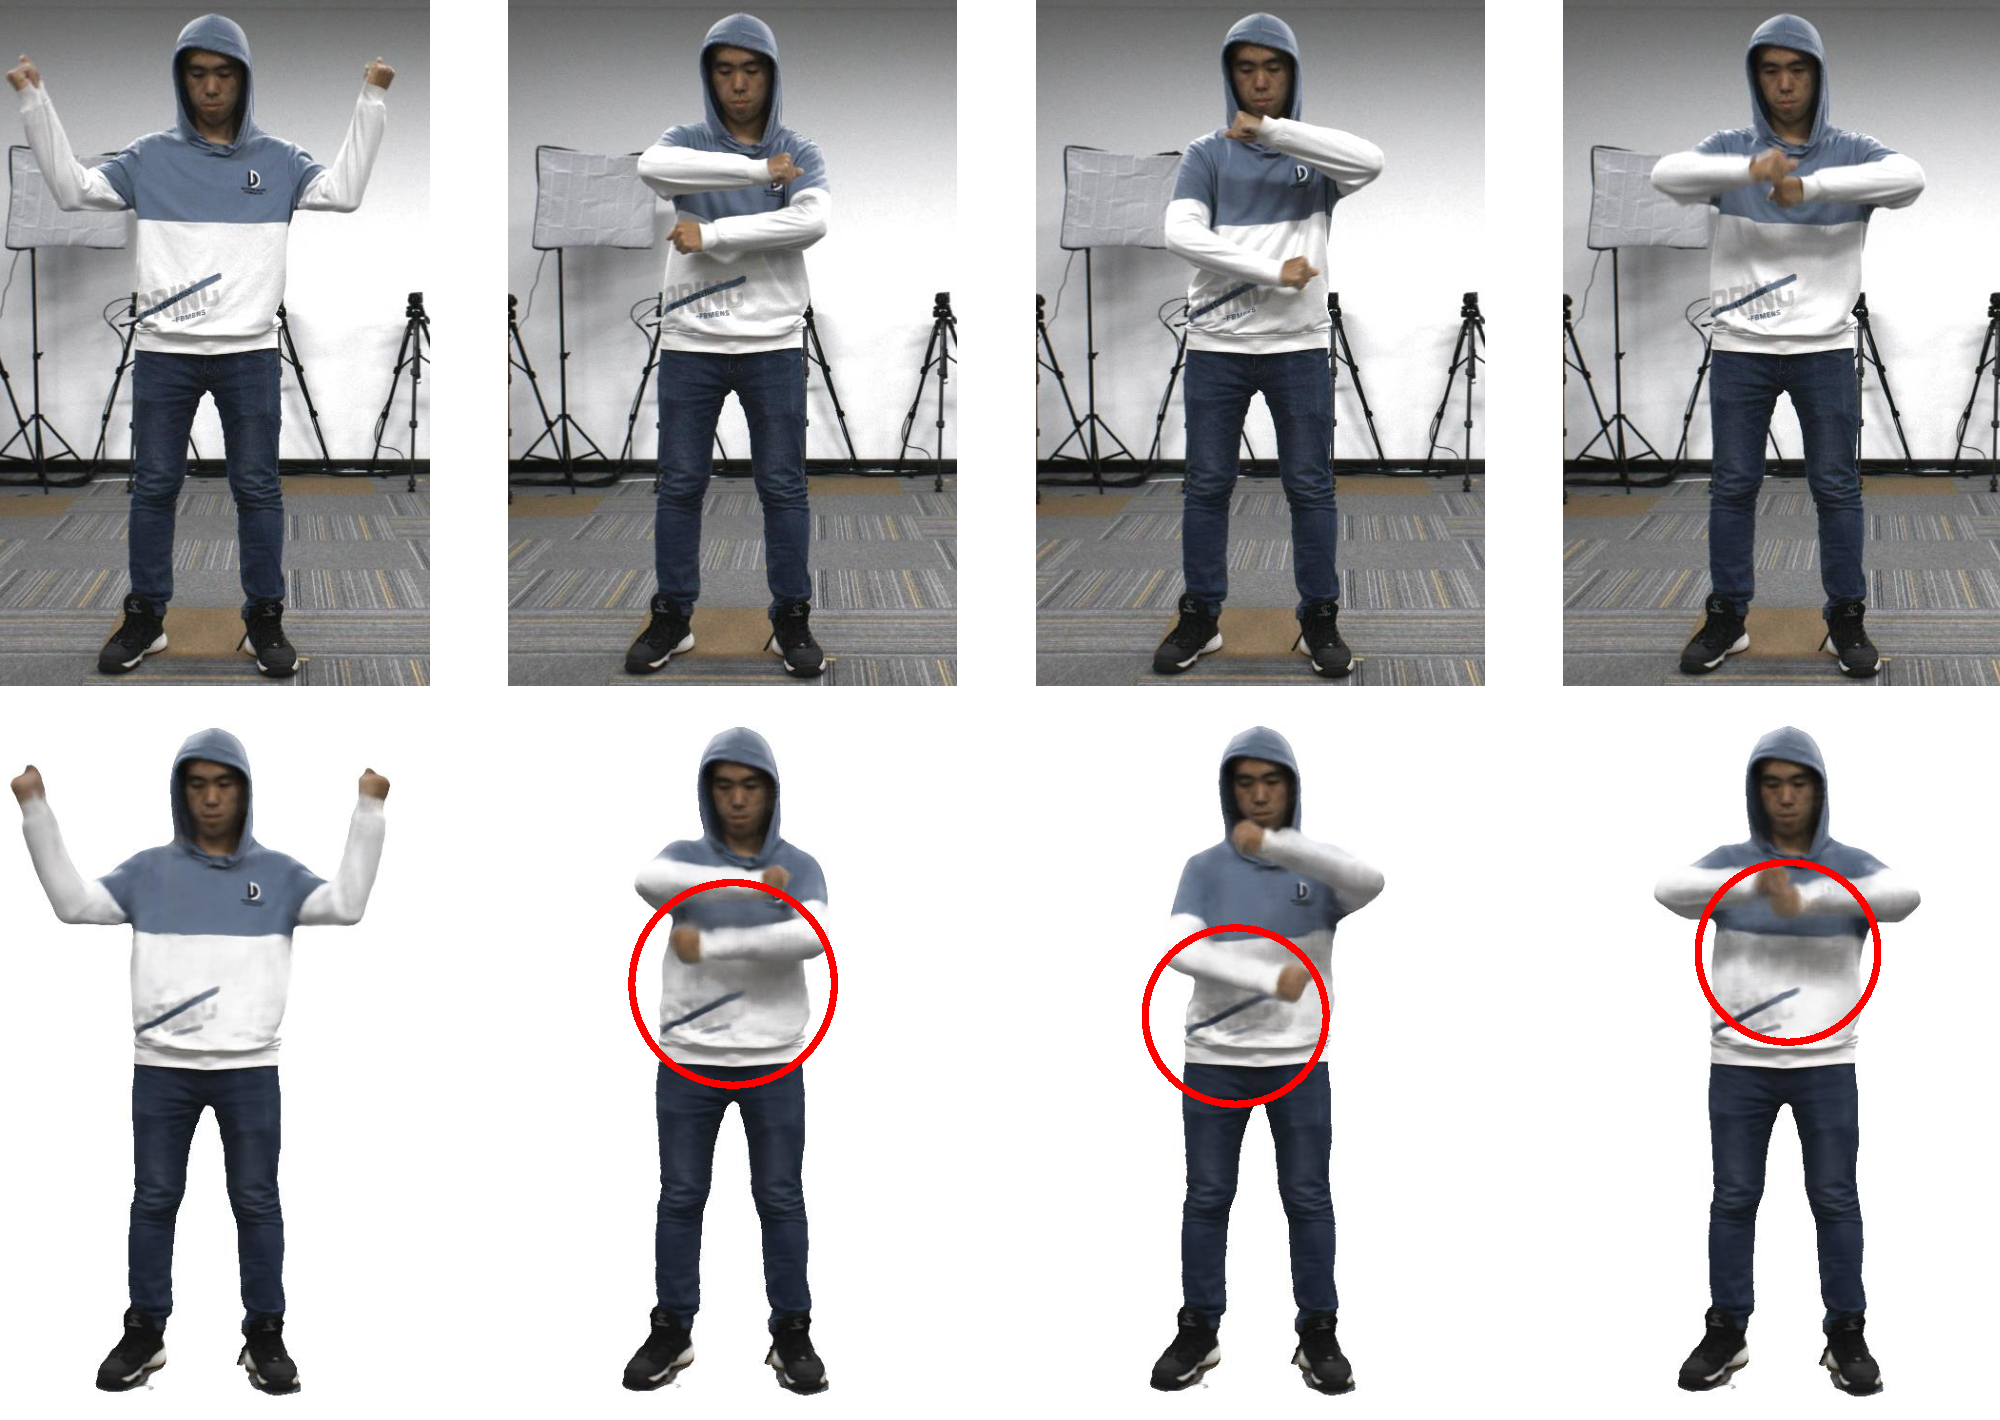
\includegraphics[width=1.0\linewidth]{shadow}
%     \caption{Our method can even learn to model the shadow effects. }
%     \label{fig:shadow}
% \end{figure}


Although we mainly use multi-view videos for evaluation, our method is also able to learn an avatar from single-view input. Fig.~\ref{fig:singleview} demonstrates the results of our method on  the PeopleSnapshot dataset~\cite{alldieck2018videoavatar}, which captures performers rotating 360 degrees in an A-pose with a monocular camera. As shown in the figure, our method can also work well with such extremely simple input, further proving its generalization capability. 


\begin{figure}
    \centering
    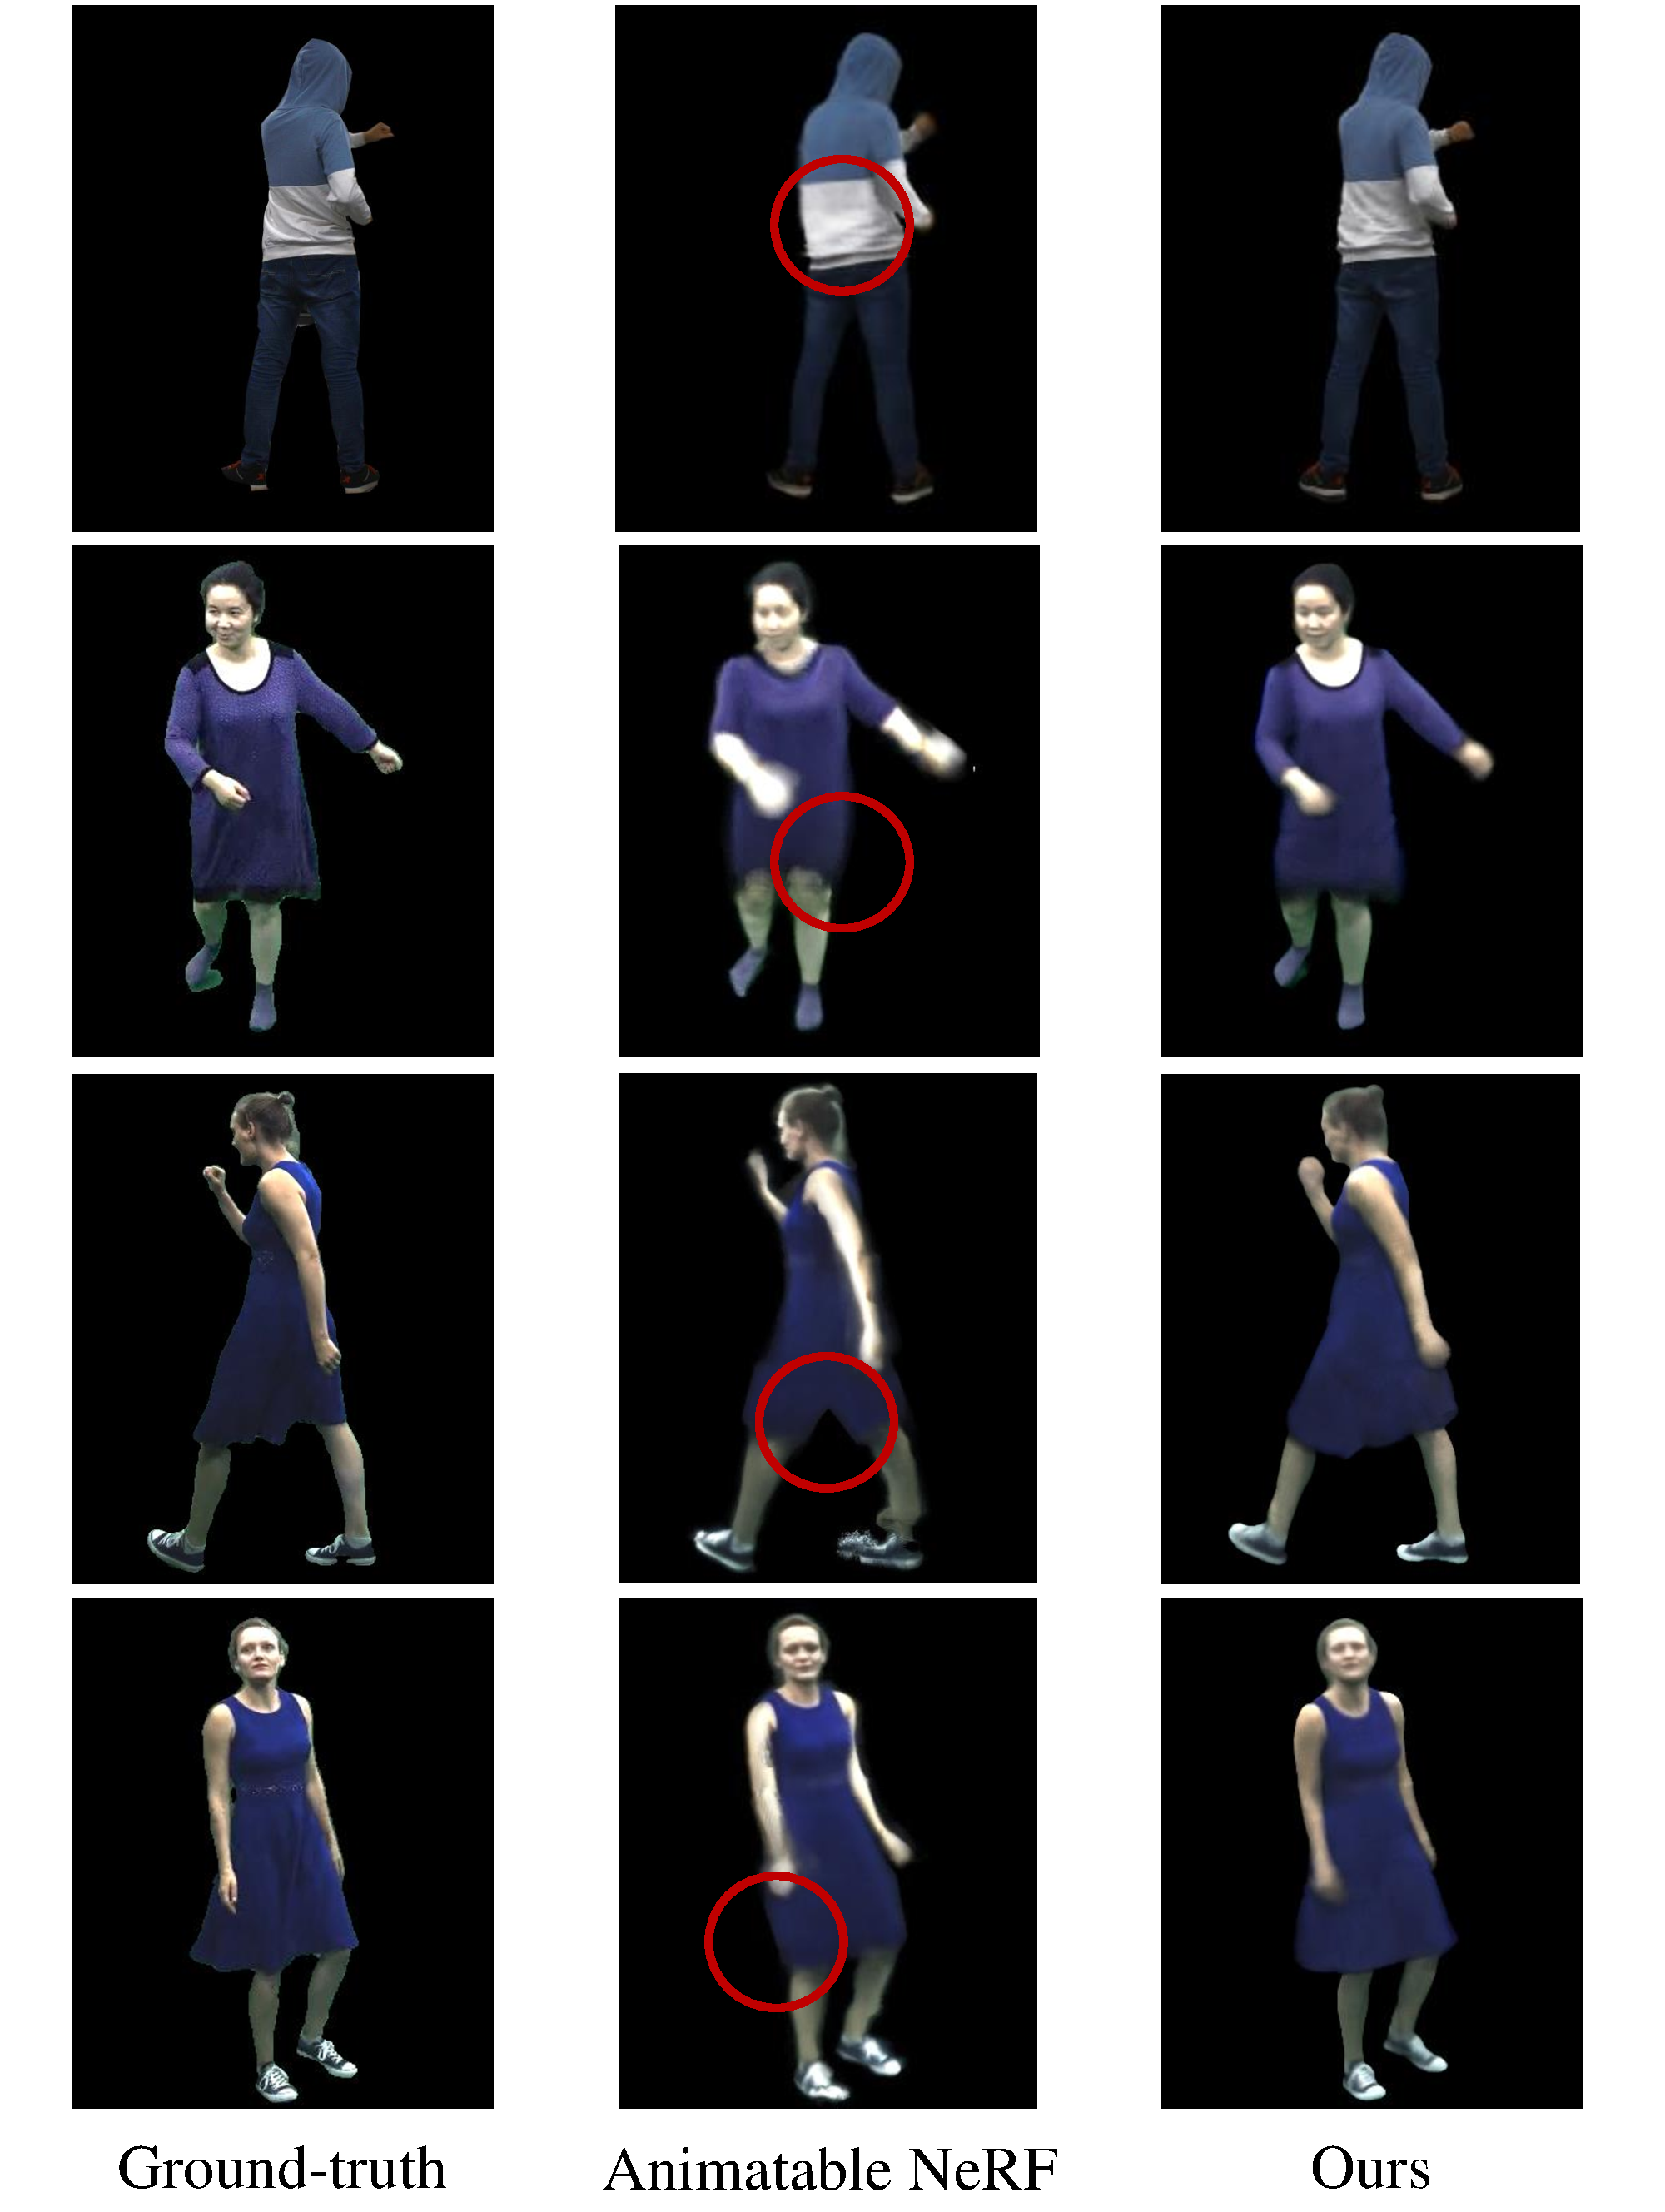
\includegraphics[width=1.0\linewidth]{anerf_comparison_cameraready}
    \caption{\textbf{Comparison against Animatable Nerf}~\cite{peng2021animatable_nerf} on novel pose synthesis. }
    \label{fig:anerf_comparison}
\end{figure}




\subsection{Comparison}
We mainly compare our method with Animatable NeRF~\cite{peng2021animatable_nerf} and Neural Body~\cite{peng2021neuralbody}. 
% We omit comparison against NHR since it has been compared in \cite{peng2021animatable_nerf}. 
% We do not compare against Neural Actors~\cite{neural_actors} and ANR~\cite{raj2020anr} because they are not open-sourced at the time of this submission, but we can claim that our method have a fundamental advantage over them in the capability of handling loose clothes (Both Neural Actors and ANR encode appearance features on the UV-map of SMPL model, which consequently restricts them from modeling various cloth topologies. ) We would love to add these comparison experiment once their code is released in the future.
% We do not compare against Neural Actors~\cite{neural_actors} because it is not open-sourced at the time of this submission, but we can claim that our method have a fundamental advantage over theirs in the capability of handling loose clothes. (\cite{neural_actors} encodes appearance features on the UV-map of SMPL model, which consequently restricts them from modeling different cloth topologies. ) We would love to add this comparison experiment once their code is released in the future.
We omit other related methods since they have been compared in \cite{peng2021animatable_nerf}. 

We first compare with Animatable NeRF~\cite{peng2021animatable_nerf} on the dataset of \cite{habermann2021realtimeDDC} and our own data. 
We split each video into training frames and testing ones, train the networks using the training frames from all views, and test the animation quality using the testing frames. 
Qualitative results are presented in  Fig.~\ref{fig:anerf_comparison}. 
Compared to \cite{peng2021animatable_nerf}, our method can produce more appearance details, and generate the non-rigid motions of dress hems. 
The numeric results in Tab.~\ref{tab:anerf_comparison} also prove that our method can achieve higher-quality results than \cite{peng2021animatable_nerf}. 


To conduct a fair comparison with Neural Body~\cite{peng2021neuralbody}, we use their dataset and follow the same protocal in their paper. In this comparison, we train our network using only 300 image frames from four views, as done in \cite{peng2021neuralbody}. We evaluate the quality of novel view synthesis for training frames and unseen body poses. 
The results in Tab.~\ref{tab:neuralbody_comparison} shows that our model achieves higher accuracy than \cite{peng2021neuralbody} in both metrics. In fact, our method performs better not only in learning appearance details like the logo, but also in generalizing to unseen poses, as shown in Fig.~\ref{fig:neuralbody_comparison}. We also report the numeric results of Animatable NeRF~\cite{peng2021animatable_nerf} in Tab.~\ref{tab:neuralbody_comparison} for completeness. 


\begin{table}[t]
\centering
    \caption{Quantitative comparison with Animatable NeRF~\cite{peng2021animatable_nerf} in terms of novel pose synthesis.  }
  % \scriptsize
    \scriptsize
    \begin{threeparttable}
    \begin{tabular}{lcccc}
        \toprule
         & \multicolumn{2}{c}{PSNR ($\uparrow$)} & \multicolumn{2}{c}{SSIM ($\uparrow$)}                \\
        \cmidrule(r){2-3} \cmidrule(r){4-5} 
        Case $\backslash$ Method    & \cite{peng2021animatable_nerf} & Ours & \cite{peng2021animatable_nerf} & Ours \\
        \midrule 
        Hoody & 22.43 & \textbf{24.94} & 0.893 & \textbf{0.928} \\
        Jacket & 24.30 & \textbf{25.24} & 0.909 & \textbf{0.927} \\
        Dress1  & 19.52 & \textbf{23.43} & 0.848 & \textbf{0.891} \\
        Dress2 & 20.49 & \textbf{22.19} & 0.877 & \textbf{0.900} \\
        \bottomrule
    \end{tabular}
    % \begin{tablenotes} 
    %     \scriptsize
    %     \item[$\ast$] Based on encoder-decoder network architectures. 
    %     \item[$\dagger$] Based on auto-decoder network architectures and requires latent optimization during testing.  
    % \end{tablenotes}
    \end{threeparttable}
    \vspace{2pt}
    \label{tab:anerf_comparison}
\end{table}



\begin{table}[t]
  \centering
  \scriptsize
  \caption{Quantitative comparison with Neural Body~\cite{peng2021neuralbody} and Animatable NeRF~\cite{peng2021animatable_nerf} on ZJU-MoCap dataset.}
    \begin{tabular}{ccrrrrrr}
    \toprule
          &       & \multicolumn{3}{c}{PSNR ($\uparrow$)} & \multicolumn{3}{c}{SSIM ($\uparrow$)} \\
    \cmidrule(r){3-5} \cmidrule(r){6-8} 
    \multicolumn{1}{c}{ID} & Pose Type & \multicolumn{1}{c}{\cite{peng2021neuralbody}} & \multicolumn{1}{c}{\cite{peng2021animatable_nerf}} & \multicolumn{1}{c}{Ours} & \multicolumn{1}{c}{\cite{peng2021neuralbody}} & \multicolumn{1}{c}{\cite{peng2021animatable_nerf}} & \multicolumn{1}{c}{Ours} \\
    \midrule 
    \multirow{2}{*}{387} & Seen  & 25.79 & 24.38     & \textbf{28.32}     & 0.928 & 0.903     & \textbf{0.953} \\
          & Unseen & 21.60 & 21.29     & \textbf{23.61}     & 0.870  & 0.860     & \textbf{0.905} \\
    \midrule 
    \multirow{2}{*}{392} & Seen  & 29.44 & 27.43 & \textbf{30.79} & 0.946 & 0.919 & \textbf{0.958} \\
          & Unseen & 25.76 & 24.59 & \textbf{26.74} & 0.909 & 0.889 & \textbf{0.927} \\
    \bottomrule
    \end{tabular}%
  \label{tab:neuralbody_comparison}%
\end{table}%


\begin{figure}
    \centering
    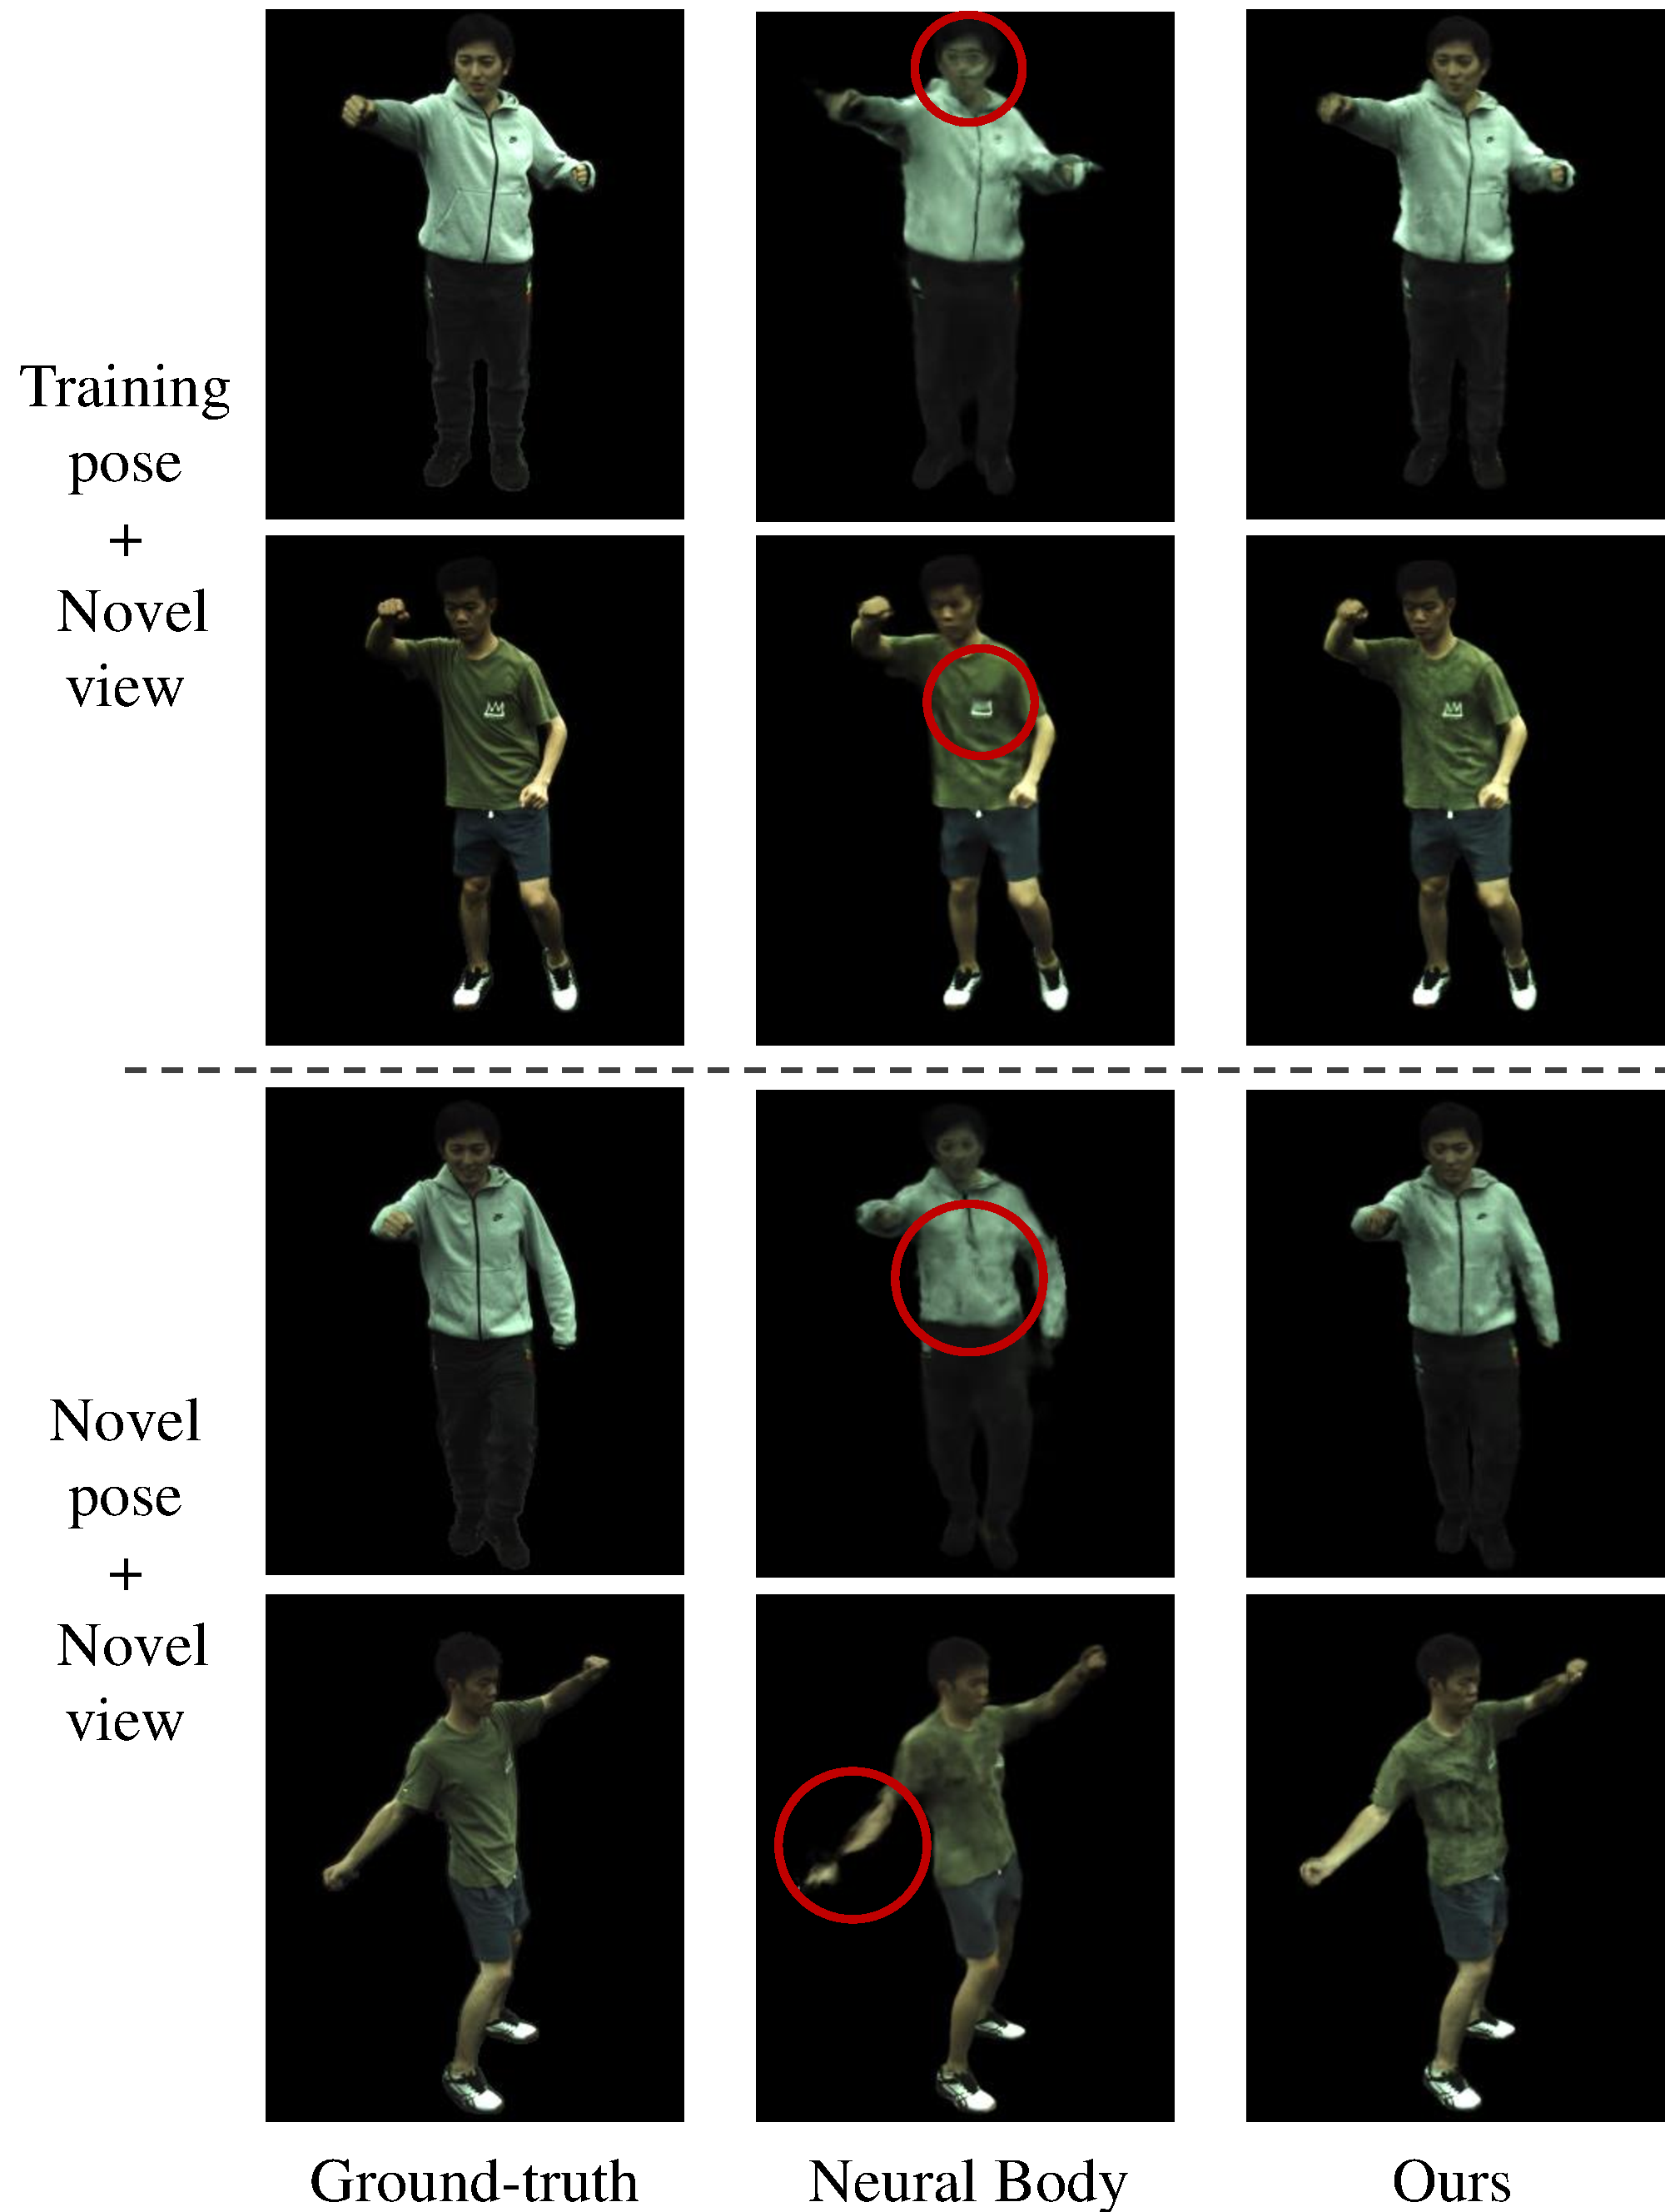
\includegraphics[width=1.0\linewidth]{neuralbody_comparison}
    \caption{\textbf{Comparison against Neural Body}~\cite{peng2021neuralbody} in terms of both novel view synthesis and pose generation. Zoom in for better view.}
    \label{fig:neuralbody_comparison}
\end{figure}



\subsection{Ablation Study}
\label{sec:experiments:evaluation}
In this subsection, we conduct three qualitative ablation experiments on the main components of our method design. We present the quantitative results as well as some additional experiments in the \textit{Supp.Mat.}. 

\noindent\textbf{Node-related variables.} 
To understand the effect of the node-related variables in our method, we take the trained model for a dress sequence and conduct experiment on it. Specifically, we render the images of training poses under three circumstances, \textit{i.e.}, 1) without node residual translations or dynamic detail embeddings, 2) with node residual translations but without dynamic detail embeddings, and 3) with both node translations and detail embeddings. 
The results are shown in Fig.~\ref{fig:eval_node_effect}. 
As the figure shows, when the node residual translations and the dynamic detail embeddings are both disabled, the model only recovers the articulated motions and fails to render the correct shape of the moving character. With solely the node residual translation enabled, the non-rigid deformation of the dress hem can be recovered, but the shading on the facial area is not consistent with the image evidence. Only with both the node residual translation and the dynamic detail embeddings enabled can all appearance details be faithfully reconstructed. 


% \begin{figure}
%     \centering
%     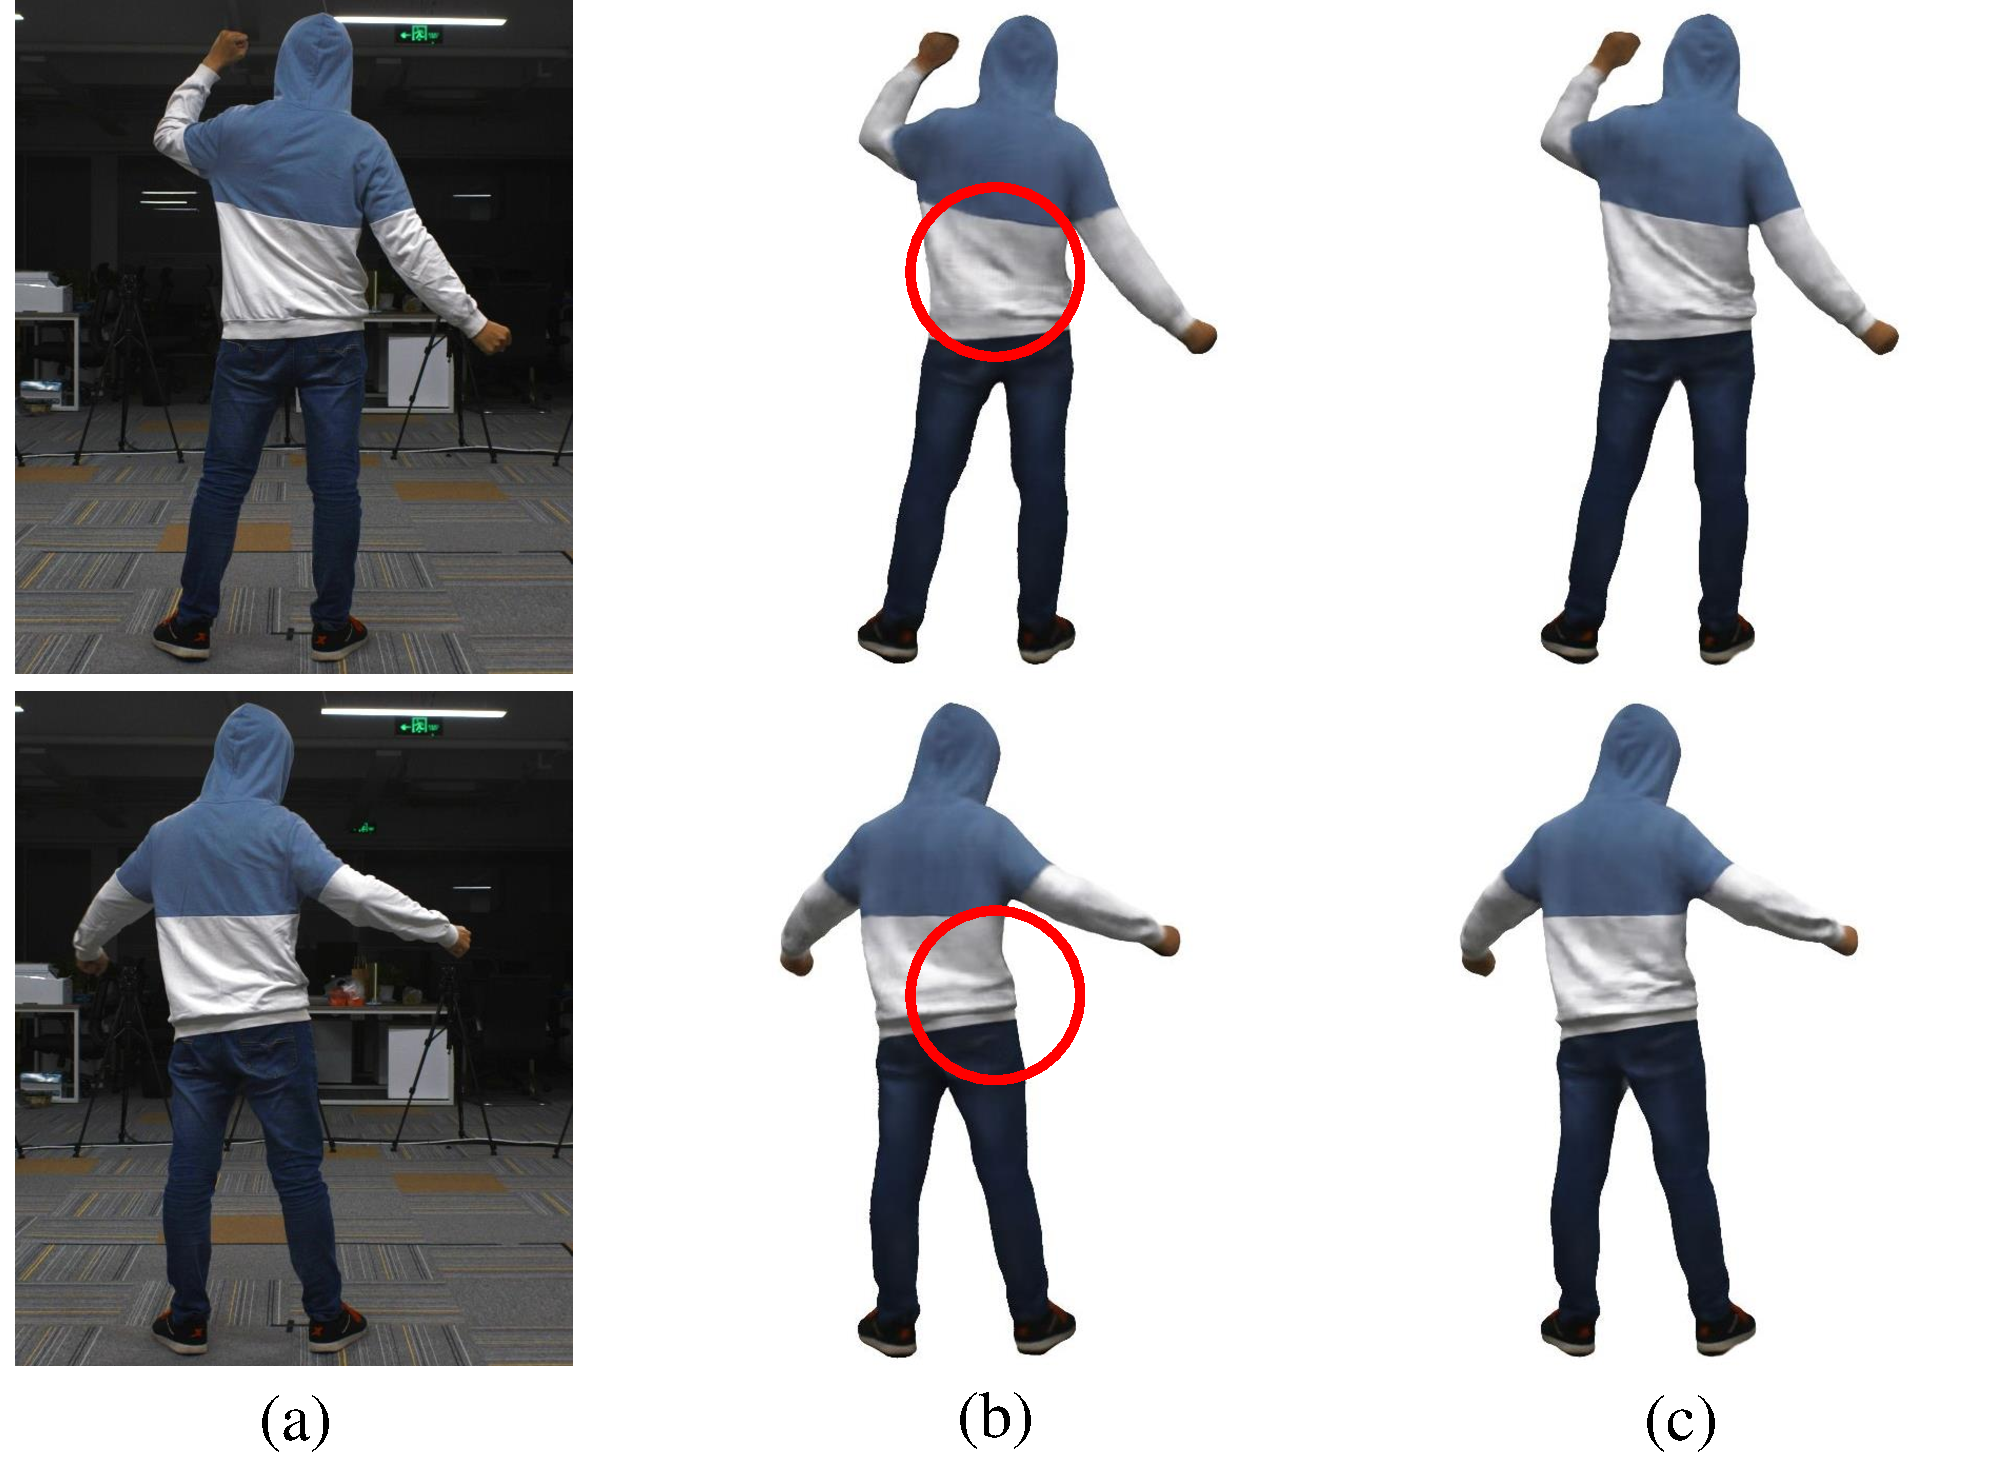
\includegraphics[width=1.0\linewidth]{eval_vae}
%     \caption{\textbf{Evaluation of our cVAE design.} We replace the cVAE with a determinstic regression network, and compare the reconstruction results of training frames. (a) Ground-truth. (b) Results by the deterministic baseline. (c) Results by the proposed network.  }
%     \label{fig:eval_cvae}
% \end{figure}

\begin{figure}
    \centering
    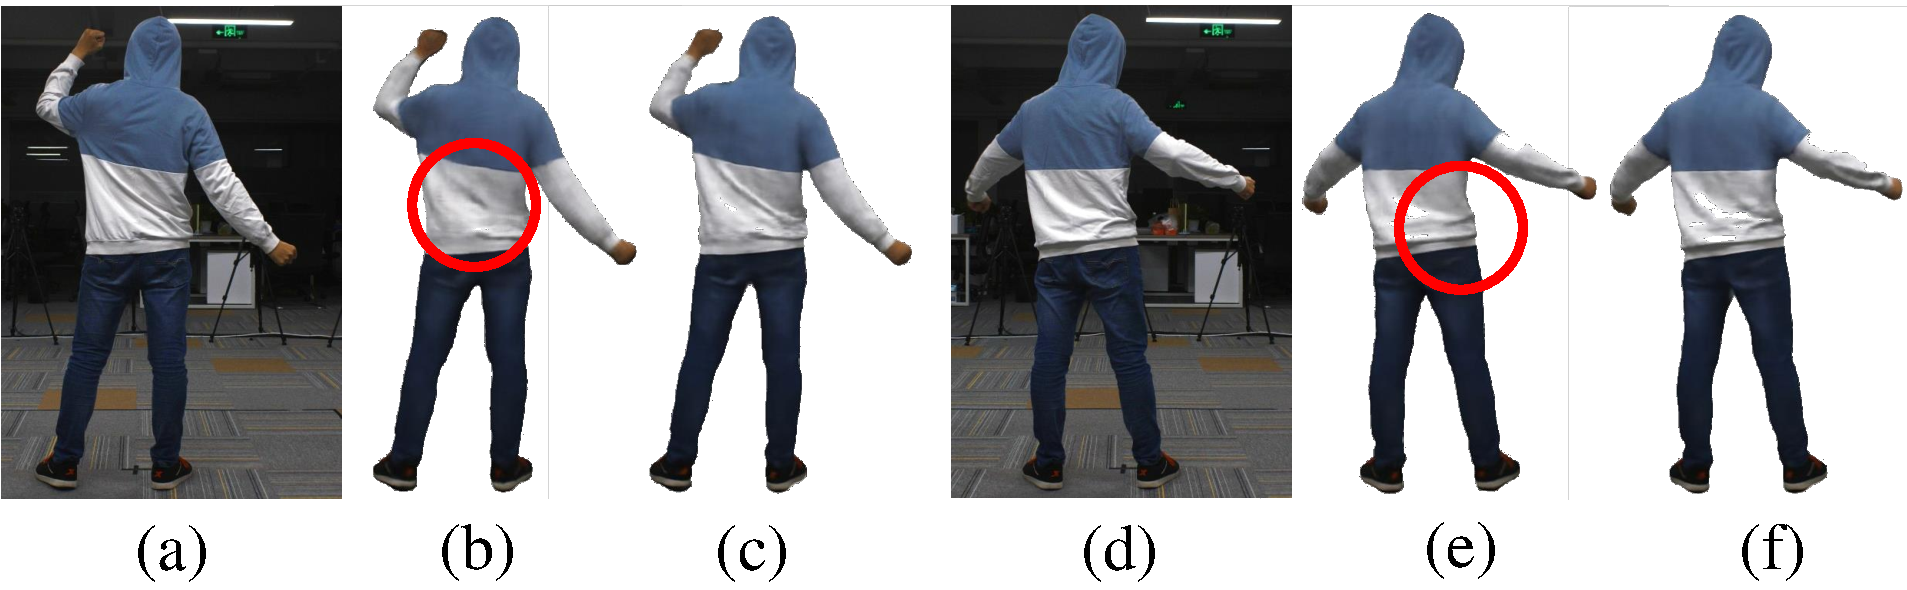
\includegraphics[width=1.0\linewidth]{eval_vae_small}
    \caption{\textbf{Evaluation of our cVAE design.} We replace the cVAE with a determinstic regression network, and compare the reconstruction results of training frames. (a,d) Ground-truth. (b,e) Results by the deterministic baseline. (c,f) Our results.  }
    \label{fig:eval_cvae}
\end{figure}


\noindent\textbf{cVAE. }
We evaluate our choice of cVAE-based architecture by replacing it with a deterministic network that directly regresses the node-related variables from body poses. This baseline network is trained under the same setting as our proposed model. 
We render the images for training frames in order to compare the performance of data fitting, and the results are  presented in Fig.~\ref{fig:eval_cvae}. 
Not surprisingly, naively learning a mapping from pose parameters to the node-related variables, without specifically account for the potential one-to-many mapping problem, will produce averaged appearance and fail to recover the dynamic garment wrinkles even for training images. In contrast, our method can fit to training data much better than the baseline method, consequently enabling realistic animation and rendering. 


\begin{figure}
    \centering
    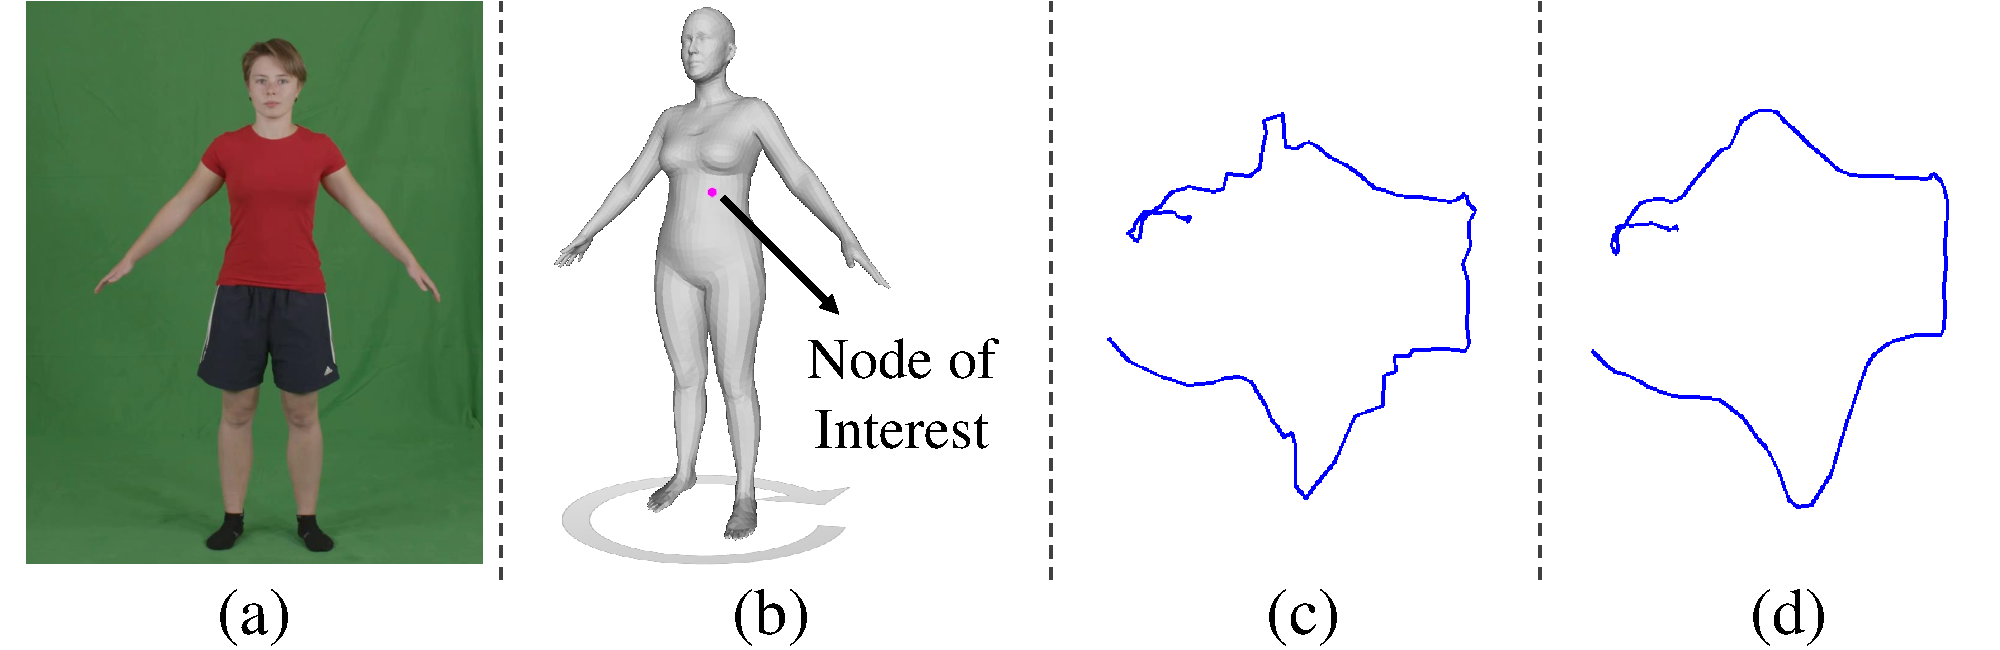
\includegraphics[width=1.0\linewidth]{eval_time}
    \caption{\textbf{Evaluation of the time instant input.} We replace the time stamp input with learnable per-frame latent codes and compare the trajectory of nodes. (a) Training video. (b) The node of which we visualize the trajectory. (c) Node trajectory using learnable latent codes. (d) Node trajectory using the proposed method. }
    \label{fig:eval_time}
\end{figure}



\noindent\textbf{Time stamp input. }
There exist other options that can be used as the cVAE input for resolving the one-to-many mapping problem. For instance, we can use learnable per-frame latent embeddings. The motivation behind our choice of time stamp is that, the low-frequency bias in MLPs can ensure temporal smoothness of the node-related variables, especially for node residual translations. In this way, we avoid the need for an additional loss of temporal smoothness. To validate this motivation, we conduct an ablation study where we replace the time stamp input with learnable latent embeddings. Then we compare the node trajectories as in Fig.~\ref{fig:eval_time}. As shown by the results, without explicitly constraining the temporal smoothness, the baseline method learns noisy node motions, while the trajectory of our method is much more smooth and physically plausible. 


